\documentclass{article}
\usepackage{amsmath}
\usepackage{amssymb}
\usepackage{graphicx}
\usepackage{hyperref}
\usepackage[version=4]{mhchem}

\title{Problem 3}
\date{}

\begin{document}
\maketitle

\section*{Problem}
As shown in the figure, \(A B C D\) is a trapezoid with the bases \(A B\) and \(D C . A D=24, D C=7 . \angle C B A=45^{\circ}\) and \(\angle D A B=\) \(30^{\circ}\). Find the length of \(A B\).\\
(A) \(12+\sqrt{3}\)\\
(B) 13\\
(C) \(12 \sqrt{3}\)\\
(D) \(19+12 \sqrt{3}\)\\
(E) \(24+3 \sqrt{3}\)\\
\centering
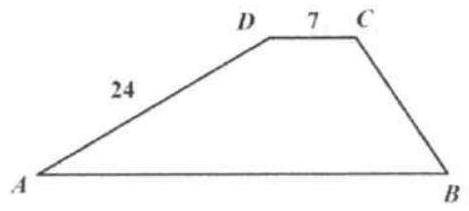
\includegraphics[width=\textwidth]{images/088(1).jpg}

\section*{Solution}
Solution not available.

\end{document}
